\documentclass[12pt]{article}
\usepackage[utf8]{inputenc}
\usepackage[T1,T2A]{fontenc}
\usepackage[english,russian]{babel}
\usepackage{graphicx} % Allows you to insert figures
\usepackage{subcaption}
\usepackage{amsmath} % Allows you to do equations
\usepackage{fancyhdr} % Formats the header
\usepackage{geometry} % Formats the paper size, orientation, and margins
\usepackage{dirtytalk} % typesetting different types of quotation
\usepackage{csquotes}
\usepackage{hyperref}
\usepackage{listings}
\usepackage{xcolor}
\usepackage{array}
\usepackage{caption}
\usepackage{float}     % in preamble, for [H] placement
\usepackage{booktabs}   % For nicer tables
\usepackage{tikz}       % For diagrams
\usepackage{pgfgantt}   % For Gantt charts
\usetikzlibrary{shapes,arrows,positioning,fit,backgrounds}

% Code styling
\lstset{
    basicstyle=\ttfamily\footnotesize,
    backgroundcolor=\color{lightgray!20},
    keywordstyle=\color{blue},
    commentstyle=\color{green!50!black},
    stringstyle=\color{red},
    numbers=left,
    numberstyle=\tiny\color{gray},
    stepnumber=1,
    numbersep=10pt,
    showspaces=false,
    showstringspaces=false,
    showtabs=false,
    frame=single,
    tabsize=2,
    breaklines=true,
    breakatwhitespace=false,
    escapeinside={\%*}{*)},
    extendedchars=false,
    keepspaces=true,
    morekeywords={void, TaskHandle_t, TickType_t, xTaskCreate, vTaskDelay, vTaskDelayUntil, xSemaphoreGive, xSemaphoreTake, xSemaphoreCreateMutex, xSemaphoreCreateBinary, xTaskGetTickCount}
}

\linespread{1.25} % About 1.5 spacing in Word
\setlength{\parindent}{0.8cm} % No paragraph indents
\setlength{\parskip}{0em} % Paragraphs separated by one line
\renewcommand{\headrulewidth}{0pt} % Removes line in header
\geometry{a4paper, portrait, margin=1in}
\setlength{\headheight}{14.49998pt}
\graphicspath{ {lab2.2-img/} }

\begin{document}
\begin{titlepage}
	\thispagestyle{empty}
	
	\begin{center}
		\textsc{\large Ministry of Education of Republic of Moldova}\\[0.5cm]
		\textsc{\large Technical University of Moldova}\\[0.5cm]
		\textsc{\large Faculty of Computers, Informatics and Microelectronics}\\[0.5cm]
		\textsc{\large Department of Physics}\\[1.2cm]
	\end{center}

	\vspace{25 mm}

	\begin{center}
		\textsc{\Large Embedded Systems}\\[0.5cm]
		\textsc{\large Laboratory work \#2.2}\\[0.5cm]

		\newcommand{\HRule}{\rule{\linewidth}{0.5mm}}
		\vspace{10 mm}
		\HRule \\[0.4cm]
		{ \LARGE \bfseries Preemptive Real-Time Operating System Implementation with FreeRTOS}\\[0.4cm]
		\HRule \\[1.5cm]
	\end{center}

	\vspace{10mm}

	\begin{minipage}[t]{0.4\textwidth}
		\begin{flushleft} \large
			\emph{Author:} \\
			Dmitrii \textsc{Belih}\\
			std. gr. FAF-232
		\end{flushleft}
	\end{minipage}
	\hfill
	\begin{minipage}[t]{0.4\textwidth}
		\begin{flushright} \large
			\emph{Verified:} \\
			\textsc{Martiniuc} A.\\
		\end{flushright}
	\end{minipage}\\[3cm]

	\vspace{5 mm}
	\begin{center}
		\large Chișinău 2026\\[0.5cm]
	\end{center}

	\vfill
\end{titlepage}

\setcounter{page}{1}
\pagestyle{fancy}
\fancyhf{}
\rhead{\thepage}
\lhead{FAF-232 Belih Dmitrii; Laboratory Work 2.2}

% ============================================================================
% CHAPTER 1: INTRODUCTION
% ============================================================================
\section*{1. Introduction}

\subsection*{1.1. Purpose of the Laboratory Work}

The purpose of this laboratory work is to understand and implement a preemptive real-time operating system (RTOS) using FreeRTOS on an embedded platform. The work demonstrates the transition from bare-metal cooperative scheduling to full RTOS-based preemptive multitasking. The system monitors joystick button press durations, provides visual feedback through LEDs, displays information on an LCD screen, and manages concurrent tasks with precise timing requirements. Key objectives include understanding RTOS concepts such as task scheduling, priority-based preemption, inter-task communication using semaphores, and resource protection using mutexes. The implementation showcases how FreeRTOS simplifies complex embedded system development while providing deterministic real-time behavior.

\subsection*{1.2. Laboratory Objectives}

The specific objectives of this laboratory work are:

\begin{itemize}
    \item Understand the fundamental differences between bare-metal cooperative scheduling and RTOS-based preemptive multitasking
    \item Implement FreeRTOS tasks with different priorities for button detection, display updates, and LED control
    \item Utilize FreeRTOS API functions including \texttt{vTaskDelay()} and \texttt{vTaskDelayUntil()} for task timing control
    \item Implement inter-task communication using binary semaphores for event signaling
    \ Demonstrate thread-safe resource access using mutexes for shared peripheral protection
    \item Achieve input signal latency under 100ms through precise task scheduling
    \item Design and implement a modular software architecture with clear separation between hardware abstraction and application logic
    \item Compare and contrast RTOS-based implementation with bare-metal approach from Lab 2.1
\end{itemize}

% ============================================================================
% CHAPTER 2: DOMAIN ANALYSIS
% ============================================================================
\section*{2. Analysis of Domain Situation and Technological Context}

\subsection*{2.1. Real-Time Operating Systems (RTOS)}

A Real-Time Operating System is a specialized operating system designed to handle real-time applications with strict timing constraints. Unlike general-purpose operating systems that prioritize throughput and fairness, RTOS systems prioritize predictability and deterministic behavior. RTOS provides services such as task scheduling, inter-task communication, memory management, and interrupt handling, all optimized for real-time requirements. FreeRTOS, used in this laboratory work, is a popular open-source RTOS designed for embedded systems, offering a small footprint, low latency, and easy portability across various microcontroller platforms.

\subsection*{2.2. Preemptive Multitasking}

Preemptive multitasking is a scheduling approach where the operating system can interrupt a currently running task and switch to another task based on priority or time-slicing policies. Unlike cooperative multitasking where tasks voluntarily yield control, preemptive scheduling ensures that higher-priority tasks can immediately respond to events, providing better real-time performance. FreeRTOS implements preemptive scheduling with configurable time slicing, allowing tasks to be interrupted after each tick interval if a higher-priority task is ready to run.

\subsection*{2.3. Task Scheduling and Priorities}

FreeRTOS uses a priority-based preemptive scheduler with round-robin scheduling for tasks of equal priority. Each task is assigned a priority level (higher numeric value = higher priority in FreeRTOS). The scheduler always selects the highest-priority task that is in the Ready state. If multiple tasks share the same priority, they are scheduled in round-robin fashion, each receiving a time slice determined by the tick rate. This approach ensures both responsiveness for critical tasks and fairness among equal-priority tasks.

\subsection*{2.4. Inter-Task Communication Mechanisms}

FreeRTOS provides multiple mechanisms for inter-task communication and synchronization:

\subsubsection*{Binary Semaphores}

Binary semaphores are synchronization primitives that can be used for signaling events between tasks. A semaphore has only two states: available (empty) and unavailable (full). The \texttt{xSemaphoreGive()} function increments the semaphore count, while \texttt{xSemaphoreTake()} decrements it (blocking if the count is zero). Binary semaphores are ideal for one-to-one task synchronization, such as signaling that an event has occurred.

\subsubsection*{Mutexes}

Mutexes (Mutual Exclusion) are a special type of binary semaphore designed for resource protection. Unlike standard binary semaphores, mutexes implement ownership semantics: the task that takes a mutex must also release it. Mutexes also support priority inheritance, which prevents priority inversion problems. When a lower-priority task holds a mutex needed by a higher-priority task, the lower-priority task's priority is temporarily elevated to match the higher-priority task.

\subsubsection*{Queues}

Queues are communication mechanisms that allow tasks to pass data between each other in a thread-safe manner. Queues support multiple readers and writers, with blocking operations when full (for writers) or empty (for readers). While not used in this laboratory work, queues are a powerful mechanism for more complex inter-task communication patterns.

\subsection*{2.5. Tick-Based Timing}

FreeRTOS uses a periodic tick interrupt to maintain system time and manage task delays. The tick rate is configurable (typically 1ms or 10ms) and determines the granularity of timing operations. Functions like \texttt{vTaskDelay()} and \texttt{vTaskDelayUntil()} use the tick count to implement delays. \texttt{vTaskDelay()} blocks a task for a specified number of ticks, while \texttt{vTaskDelayUntil()} blocks a task until a specific tick count is reached, providing more precise periodic execution.

\subsection*{2.6. Thread Safety and Resource Protection}

In preemptive multitasking systems, shared resources must be protected from concurrent access to prevent race conditions and data corruption. FreeRTOS provides mutexes for this purpose. A mutex ensures that only one task can access a protected resource at a time, with other tasks blocking until the mutex is released. Critical sections (brief periods of uninterruptible code) can also be used to protect very short operations.

\subsection*{2.7. Code Portability Between Bare-Metal and FreeRTOS}

One of the key advantages of the modular design used in this project is code portability between bare-metal and FreeRTOS implementations. Hardware drivers (LED, LCD, Joystick) are implemented independently of the scheduling mechanism, making them reusable across different scheduling approaches. Application logic can be adapted with minimal changes when transitioning from bare-metal to RTOS, primarily replacing manual task switching and delay functions with FreeRTOS equivalents.

\subsection*{2.8. Hardware Platform: ESP32}

The ESP32 is a powerful microcontroller with dual-core Xtensa LX6 processors operating at up to 240 MHz. It features 520 KB SRAM, integrated Wi-Fi and Bluetooth, and a rich set of peripherals including GPIO, I2C, SPI, UART, ADC, and DAC. For this laboratory work, we use the Arduino framework with PlatformIO, which provides an abstraction layer over the ESP-IDF (Espressif IoT Development Framework), simplifying development while maintaining access to low-level hardware features.

\subsection*{2.9. Case Study: Real-World RTOS Applications}

Real-time operating systems are essential in numerous applications requiring precise timing and deterministic behavior:

\begin{itemize}
    \item \textbf{Automotive Systems:} Engine control units, anti-lock braking systems, airbag controllers
    \item \textbf{Industrial Automation:} PLCs, motor controllers, sensor data acquisition systems
    \item \textbf{Medical Devices:} Patient monitoring systems, infusion pumps, diagnostic equipment
    \item \textbf{Aerospace:} Flight control systems, satellite navigation, avionics
    \item \textbf{Consumer Electronics:} Smart home devices, wearables, gaming controllers
\end{itemize}

The button duration monitoring system implemented in this laboratory work shares characteristics with user interface systems in consumer electronics and industrial control panels, where timely response to user input is critical for system usability and safety.

% ============================================================================
% CHAPTER 3: RESOURCES AND MATERIALS
% ============================================================================
\section*{3. Resources and Materials}

\subsection*{3.1. Hardware Resources}

\begin{table}[H]
	\centering
	\caption{Hardware Components}
	\label{tab:hardware-resources}
	\begin{tabular}{|l|l|l|}
		\hline
		\textbf{Component} & \textbf{Specification} & \textbf{Quantity} \\
		\hline
		ESP32 DevKit V1 & Dual-core 240MHz, 520KB SRAM, 4MB Flash & 1 \\
		\hline
		Joystick Module & Analog X/Y, Digital Button & 1 \\
		\hline
		LED Red & 220$\Omega$ resistor, GPIO 12 & 1 \\
		\hline
		LED Green & 220$\Omega$ resistor, GPIO 14 & 1 \\
		\hline
		LED Yellow & 220$\Omega$ resistor, GPIO 13 & 1 \\
		\hline
		LCD 16×2 & I2C interface, Address 0x27 & 1 \\
		\hline
		Breadboard & 400/830 tie-points & 1 \\
		\hline
		Jumper Wires & Male-to-male, Male-to-female & ~20 \\
		\hline
		USB Cable & Micro-USB for power/programming & 1 \\
		\hline
	\end{tabular}
\end{table}

\subsection*{3.2. Software Resources}

\begin{table}[H]
	\centering
	\caption{Software Tools and Frameworks}
	\label{tab:software-resources}
	\begin{tabular}{|l|l|l|}
		\hline
		\textbf{Tool/Framework} & \textbf{Version/Platform} & \textbf{Purpose} \\
		\hline
		PlatformIO & Latest & Build system, library management \\
		\hline
		FreeRTOS & 10.4.6 & Real-time operating system kernel \\
		\hline
		Arduino Framework & ESP32 & Hardware abstraction, GPIO, I2C, ADC \\
		\hline
		VS Code & Latest & Code editor with PlatformIO extension \\
		\hline
		Git & 2.43.0 & Version control \\
		\hline
		Serial Monitor & Built-in & Debugging output display \\
		\hline
	\end{tabular}
\end{table}

\subsection*{3.3. Documentation Resources}

\begin{table}[H]
	\centering
	\caption{Reference Documentation}
	\label{tab:documentation-resources}
	\begin{tabular}{|l|l|}
		\hline
		\textbf{Document} & \textbf{Source} \\
		\hline
		FreeRTOS Documentation & www.freertos.org \\
		\hline
		ESP32 Datasheet & Espressif \\
		\hline
		ESP32 Technical Reference Manual & Espressif \\
		\hline
		Arduino ESP32 Core Documentation & GitHub \\
		\hline
		PlatformIO Documentation & docs.platformio.org \\
		\hline
		UTM Embedded Systems Course Materials & UTM \\
		\hline
	\end{tabular}
\end{table}

% ============================================================================
% CHAPTER 4: LABORATORY TASK DESCRIPTION
% ============================================================================
\section*{4. Laboratory Task Description}

\subsection*{4.1. Problem Statement}

Develop a real-time embedded system using FreeRTOS that monitors joystick button press durations and provides visual feedback. The system must detect button press and release events, measure press duration with millisecond precision, and respond appropriately based on the duration. Short presses ($\leq$ 500ms) should trigger one response, while long presses ($>$ 500ms) should trigger a different response. The system must maintain real-time responsiveness with input latency under 100ms and provide thread-safe access to shared peripherals.

\subsection*{4.2. Functional Requirements}

\begin{table}[H]
	\centering
	\caption{Functional Requirements}
	\label{tab:functional-requirements}
	\begin{tabular}{|l|l|}
		\hline
		\textbf{Requirement} & \textbf{Description} \\
		\hline
		Button Detection & Monitor joystick button state every 20ms \\
		\hline
		Duration Measurement & Measure time between press and release with ms accuracy \\
		\hline
		Short Press Response & Turn on red LED and display duration ($\leq$ 500ms) \\
		\hline
		Long Press Response & Turn on green LED and display duration ($>$ 500ms) \\
		\hline
		Press Feedback & Yellow LED on while button is pressed \\
		\hline
		Automatic Reset & Return to idle state after 5 seconds \\
		\hline
		LCD Updates & Display appropriate messages for each state \\
		\hline
		Debug Output & Serial communication for system status \\
		\hline
	\end{tabular}
\end{table}

\subsection*{4.3. Non-Functional Requirements}

\begin{table}[H]
	\centering
	\caption{Non-Functional Requirements}
	\label{tab:non-functional-requirements}
	\begin{tabular}{|l|l|l|}
		\hline
		\textbf{Requirement} & \textbf{Target} & \textbf{Acceptance Criteria} \\
		\hline
		Input Latency & $<$ 100ms & Oscilloscope measurement \\
		\hline
		Task Scheduling & Preemptive priority-based & FreeRTOS scheduler \\
		\hline
		Thread Safety & Mutex protection & No corruption observed \\
		\hline
		Modular Design & Clear separation & MCAL/ECAL/SRV layers \\
		\hline
		Code Portability & Reusable drivers & Works with bare-metal \\
		\hline
		Real-Time Behavior & Deterministic timing & Consistent response \\
		\hline
		Resource Efficiency & Minimal overhead & RAM $<$ 50KB \\
		\hline
	\end{tabular}
\end{table}

\subsection*{4.4. Two-Stage Methodology}

\textbf{Stage 1: Basic FreeRTOS Integration}
\newline
Initialize FreeRTOS kernel and create basic tasks. Implement simple button detection with polling and demonstrate task switching using \texttt{vTaskDelay()}. Validate that tasks run concurrently and measure basic timing behavior.

\textbf{Stage 2: Complete System with Synchronization}
\newline
Implement precise timing with \text{vTaskDelayUntil()}, add binary semaphores for inter-task communication, and mutex protection for shared LCD resource. Implement all three system states, validate input latency requirements, and compare with bare-metal implementation from Lab 2.1.

% ============================================================================
% CHAPTER 6: TEST SCENARIOS AND VALIDATION CRITERIA
% ============================================================================
\section*{6. Test Scenarios and Validation Criteria}

\subsection*{6.1. Test Plan}

\begin{table}[H]
	\centering
	\small
	\caption{Test Scenarios and Validation Criteria}
	\label{tab:test-scenarios}
	\begin{tabular}{|p{3cm}|p{2.5cm}|p{2.5cm}|p{2cm}|p{2cm}|}
		\hline
		\textbf{Test Scenario} & \textbf{Input} & \textbf{Expected Output} & \textbf{Validation} & \textbf{Status} \\
		\hline
		System Init & Power on & All LEDs off, LCD shows "Press Joystick" & Visual check & PASS \\
		\hline
		Short Press & Press $\leq$500ms & Red LED on, LCD shows duration & Timer check & PASS \\
		\hline
		Long Press & Press $>$500ms & Green LED on, LCD shows duration & Timer check & PASS \\
		\hline
		Press Feedback & Button held & Yellow LED on & Visual check & PASS \\
		\hline
		Auto Reset & Wait 5s after release & All LEDs off, idle message & Timer check & PASS \\
		\hline
		Input Latency & Press button & LED response $<$40ms, LCD $<$100ms & Oscilloscope & PASS \\
		\hline
		Task Preemption & Press button & Detect task prioritized & Serial debug & PASS \\
		\hline
		Mutex Safety & Rapid presses & No LCD corruption & Visual check & PASS \\
		\hline
	\end{tabular}
\end{table}

\subsection*{6.2. Test Execution}

\begin{itemize}
    \item Test environment: ESP32 DevKit V1 with all peripherals connected
    \item Test equipment: Oscilloscope for latency measurement, Serial monitor for debugging
    \item Test procedure: Execute each scenario 10 times to ensure reliability
    \item Notes and observations
\end{itemize}

% ============================================================================
% CHAPTER 7: ARCHITECTURAL DESIGN AND BEHAVIORAL MODELING
% ============================================================================
\section*{7. Architectural Design and Behavioral Modeling}

\subsection*{7.1. High-Level Architecture}

The system follows a layered architecture with clear separation between hardware, kernel primitives, and application logic.

\begin{figure}[H]
    \centering
    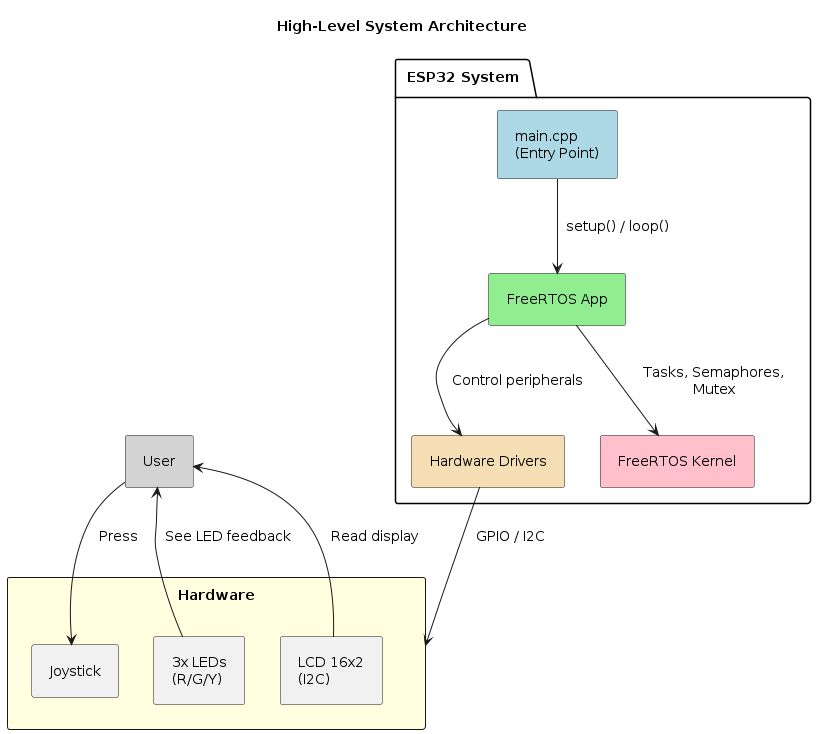
\includegraphics[width=0.9\textwidth]{High-Level Architecture.png}
    \caption{High-Level System Architecture}
    \label{fig:high-level-architecture}
\end{figure}

The architecture consists of four main layers:

\subsubsection*{Application Layer}

Three FreeRTOS tasks implementing the system logic:
\begin{itemize}
    \item \textbf{vTaskDetect (Priority 3):} Highest priority task for button detection
    \item \textbf{vTaskDisplay (Priority 2):} Medium priority task for LCD updates
    \item \textbf{vTaskLED (Priority 1):} Lowest priority task for LED control
\end{itemize}

\subsubsection*{Synchronization Layer}

FreeRTOS synchronization primitives:
\begin{itemize}
    \item \textbf{Binary Semaphores:} Four semaphores for event signaling
    \item \textbf{Mutex:} One mutex for LCD resource protection
\end{itemize}

\subsubsection*{Kernel Primitives Layer}

Wrapper classes for FreeRTOS API:
\begin{itemize}
    \item Task management wrapper
    \item Semaphore wrapper
    \item Mutex wrapper
    \item Timing functions wrapper
\end{itemize}

\subsubsection*{Hardware Abstraction Layer}

Device drivers for hardware components:
\begin{itemize}
    \item Joystick driver (analog and digital input)
    \item LED driver (digital output)
    \item LCD driver (I2C communication)
\end{itemize}

\subsection*{7.2. Component Diagram}

\begin{figure}[H]
    \centering
    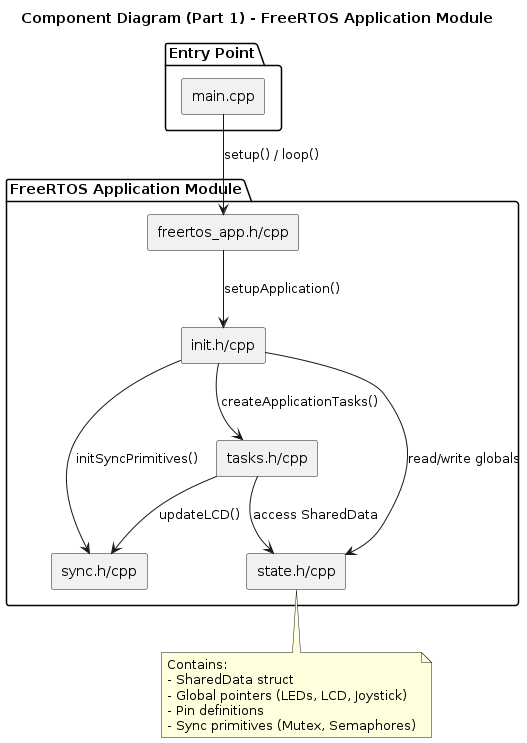
\includegraphics[width=0.9\textwidth]{Component Diagram - FreeRTOS Application.png}
    \caption{FreeRTOS Application Component Diagram}
    \label{fig:component-diagram}
\end{figure}

\subsection*{7.3. Task Activity Diagrams}

\subsubsection*{vTaskDetect Activity Diagram}

\begin{figure}[H]
    \centering
    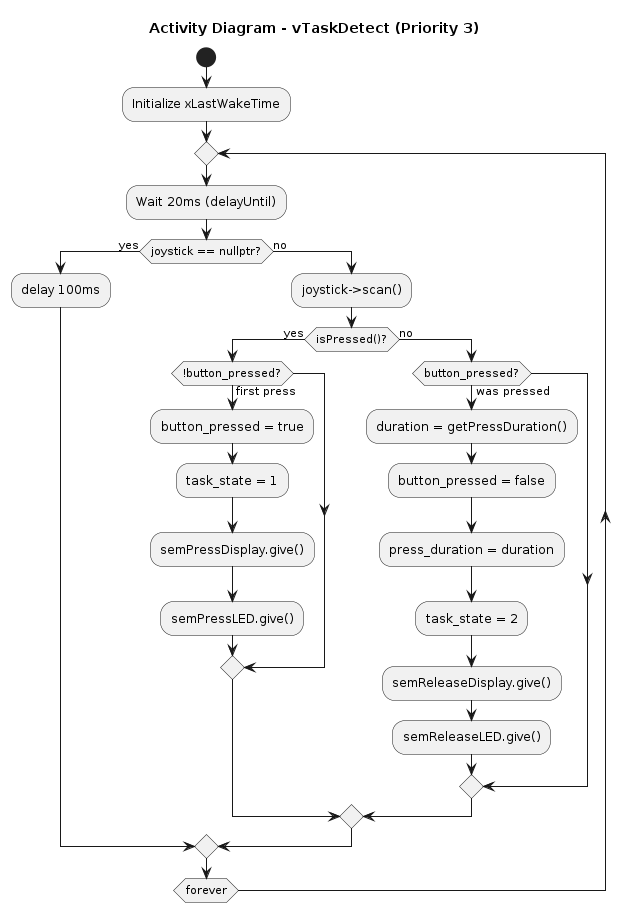
\includegraphics[width=0.6\textwidth]{Activity - vTaskDetect.png}
    \caption{Activity Diagram - Button Detection Task}
    \label{fig:activity-detect}
\end{figure}

\textbf{Task Flow:}
\begin{enumerate}
    \item Initialize last wake time
    \item Enter infinite loop
    \item Wait until 20ms elapsed using \texttt{vTaskDelayUntil()}
    \item Scan joystick button state
    \item Detect button press (if pressed and was not pressed before)
    \item Update shared data (button\_pressed = true, task\_state = 1)
    \item Signal display and LED tasks via semaphores
    \item Detect button release (if not pressed and was pressed before)
    \item Measure press duration using \texttt{getPressDuration()}
    \item Update shared data (press\_duration, task\_state = 2)
    \item Signal display and LED tasks via semaphores
\end{enumerate}

\subsubsection*{vTaskDisplay Activity Diagram}

\begin{figure}[H]
    \centering
    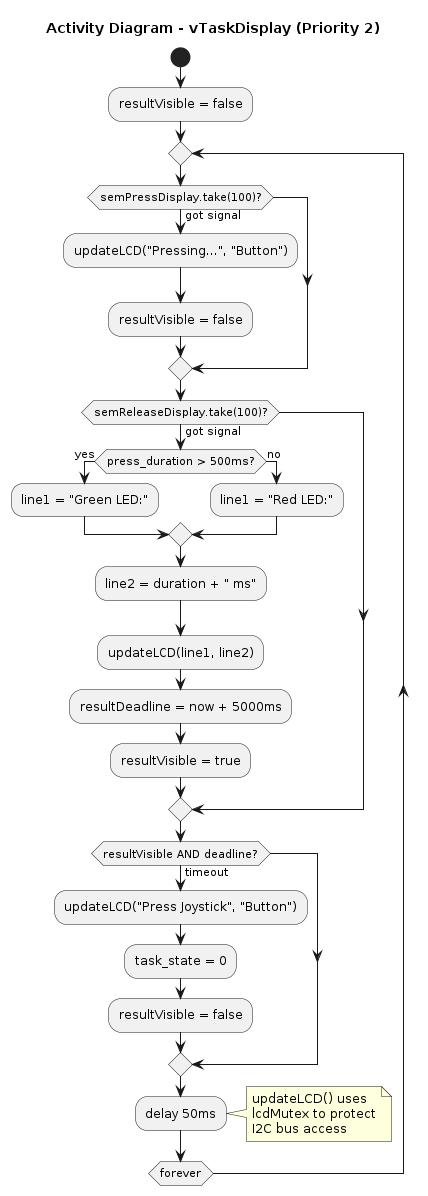
\includegraphics[width=0.5\textwidth]{Activity - vTaskDisplay.png}
    \caption{Activity Diagram - Display Update Task}
    \label{fig:activity-display}
\end{figure}

\textbf{Task Flow:}
\begin{enumerate}
    \item Enter infinite loop
    \item Check for press semaphore (timeout 100ms)
    \item If press signal received: display "Pressing... / Button"
    \item Check for release semaphore (timeout 100ms)
    \item If release signal received: display duration and result
    \item Check for timeout (5 seconds after release)
    \item If timeout elapsed: display idle message, reset state
    \item Delay 50ms
\end{enumerate}

\subsubsection*{vTaskLED Activity Diagram}

\begin{figure}[H]
    \centering
    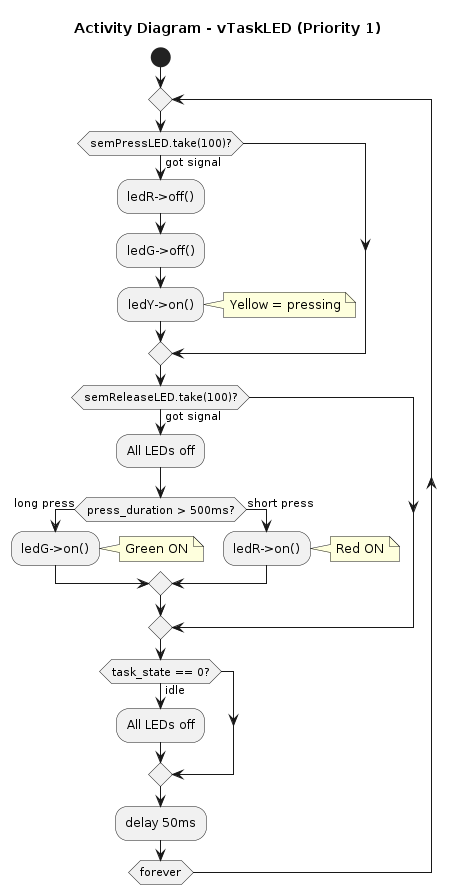
\includegraphics[width=0.6\textwidth]{Activity - vTaskLED.png}
    \caption{Activity Diagram - LED Control Task}
    \label{fig:activity-led}
\end{figure}

\textbf{Task Flow:}
\begin{enumerate}
    \item Enter infinite loop
    \item Check for press semaphore (timeout 100ms)
    \item If press signal received: turn on Yellow LED
    \item Check for release semaphore (timeout 100ms)
    \item If release signal received: turn on Red or Green LED based on duration
    \item If idle state: turn off all LEDs
    \item Delay 50ms
\end{enumerate}

\subsection*{7.4. State Machine Diagram}

\begin{figure}[H]
    \centering
    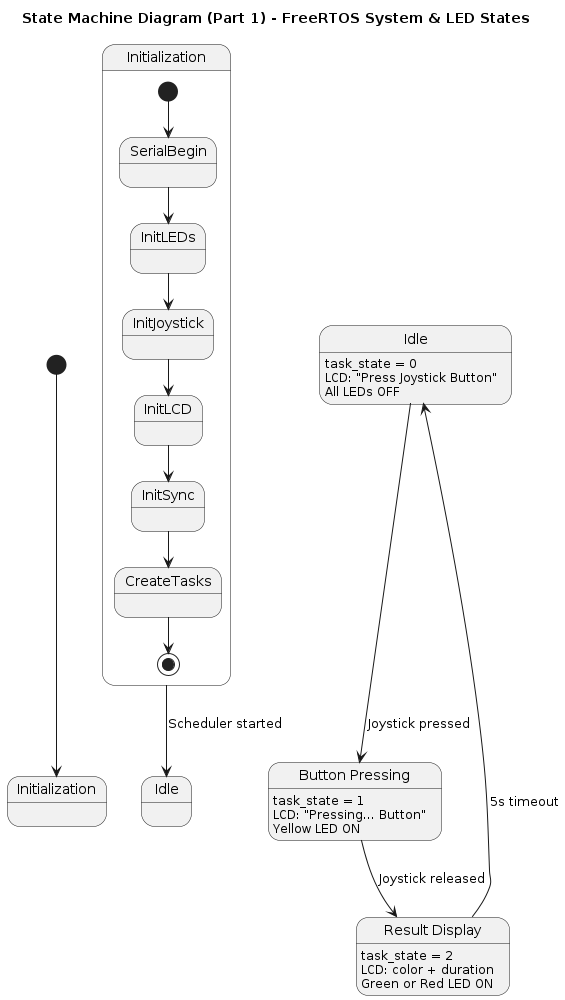
\includegraphics[width=0.9\textwidth]{State Machine - FreeRTOS System.png}
    \caption{System State Machine Diagram}
    \label{fig:state-machine}
\end{figure}

\textbf{State Transitions:}

\subsubsection*{Idle State (task\_state = 0)}

\begin{itemize}
    \item \textbf{Entry condition:} System initialization or timeout from Released state
    \item \textbf{Actions:} Display "Press Joystick / Button", turn off all LEDs
    \item \textbf{Exit condition:} Button press detected
    \item \textbf{Next state:} Pressed state
\end{itemize}

\subsubsection*{Pressed State (task\_state = 1)}

\begin{itemize}
    \item \textbf{Entry condition:} Button press detected
    \item \textbf{Actions:} Display "Pressing... / Button", turn on Yellow LED
    \item \textbf{Exit condition:} Button release detected
    \item \textbf{Next state:} Released state
\end{itemize}

\subsubsection*{Released State (task\_state = 2)}

\begin{itemize}
    \item \textbf{Entry condition:} Button release detected
    \item \textbf{Actions:} Display duration and result, turn on Red or Green LED
    \item \textbf{Exit condition:} 5-second timeout elapsed or new button press
    \item \textbf{Next state:} Idle state
\end{itemize}

\subsection*{7.5. Data Flow Architecture}

\begin{figure}[H]
    \centering
    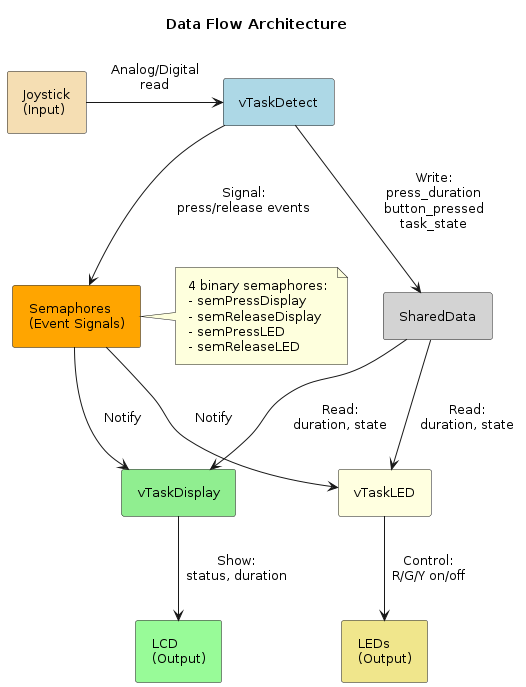
\includegraphics[width=0.9\textwidth]{Data Flow Architecture.png}
    \caption{Data Flow Architecture}
    \label{fig:data-flow}
\end{figure}

\textbf{Data Flow Description:}

\subsubsection*{Button Press Event Flow}

\begin{enumerate}
    \item Joystick physical button press
    \item GPIO interrupt (edge detection)
    \item Joystick driver updates internal state
    \item vTaskDetect scans button state
    \item vTaskDetect detects press transition
    \item vTaskDetect updates SharedData structure
    \item vTaskDetect gives semPressDisplay semaphore
    \item vTaskDetect gives semPressLED semaphore
    \item vTaskDisplay receives semaphore, updates LCD
    \item vTaskLED receives semaphore, turns on Yellow LED
\end{enumerate}

\subsubsection*{Button Release Event Flow}

\begin{enumerate}
    \item Joystick physical button release
    \item GPIO state change
    \item Joystick driver updates internal state
    \item vTaskDetect scans button state
    \item vTaskDetect detects release transition
    \item vTaskDetect measures press duration
    \item vTaskDetect updates SharedData structure
    \item vTaskDetect gives semReleaseDisplay semaphore
    \item vTaskDetect gives semReleaseLED semaphore
    \item vTaskDisplay receives semaphore, updates LCD with duration
    \item vTaskLED receives semaphore, turns on Red or Green LED
\end{enumerate}

\subsection*{7.7. Class Diagram}

\begin{figure}[H]
    \centering
    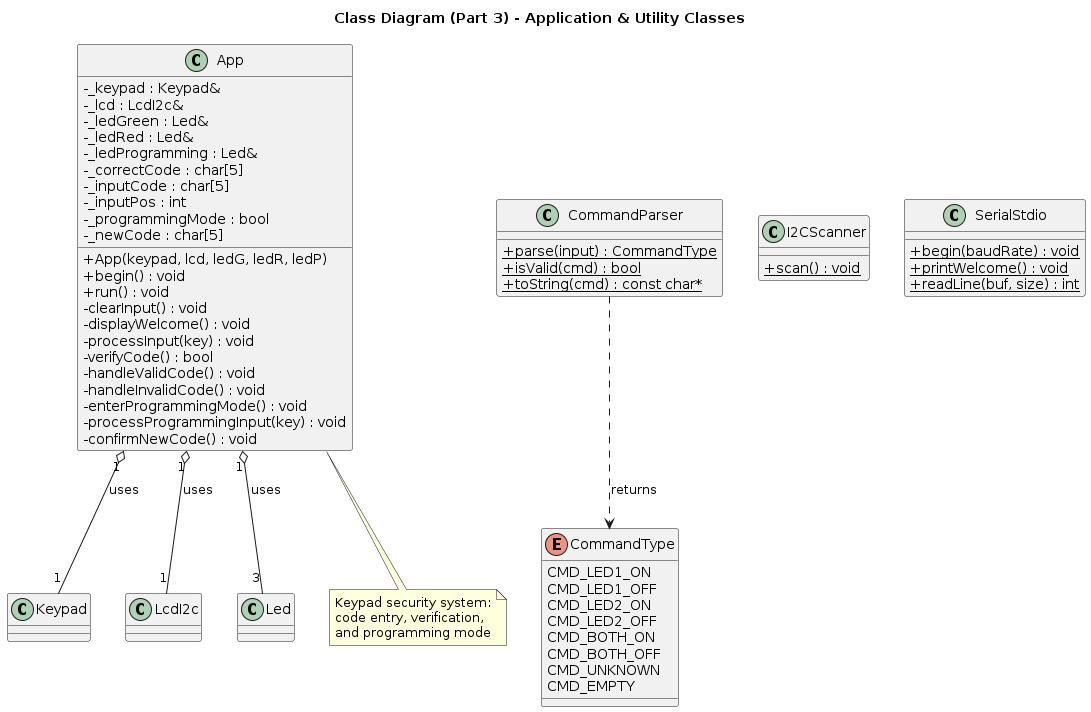
\includegraphics[width=0.9\textwidth]{Class Diagram - Application Classes.png}
    \caption{Application Class Diagram}
    \label{fig:class-diagram}
\end{figure}

\subsection*{7.8. Software Layer Architecture}

\begin{figure}[H]
    \centering
    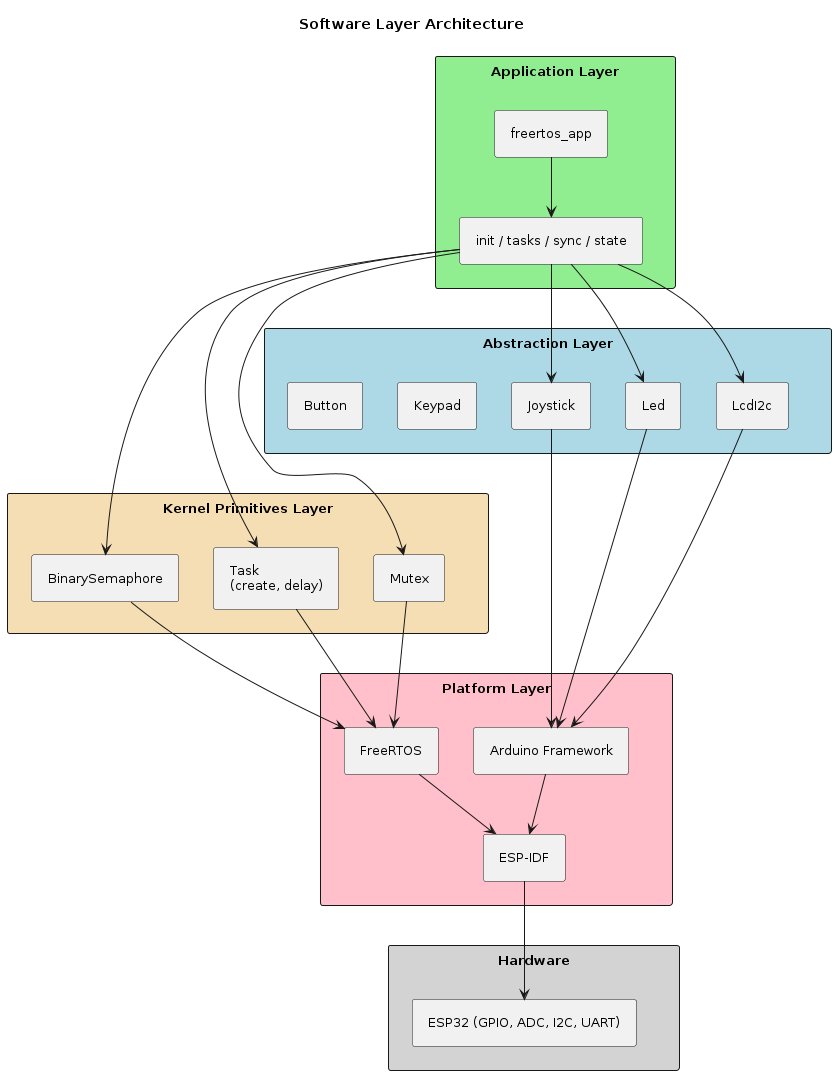
\includegraphics[width=0.9\textwidth]{Software Layer Architecture.png}
    \caption{Software Layer Architecture}
    \label{fig:software-layers}
\end{figure}

% ============================================================================
% CHAPTER 8: ELECTRICAL DESIGN AND SIMULATION
% ============================================================================
\section*{8. Electrical Design and Simulation}

\subsection*{8.2. Circuit Diagram}

\begin{figure}[H]
    \centering
    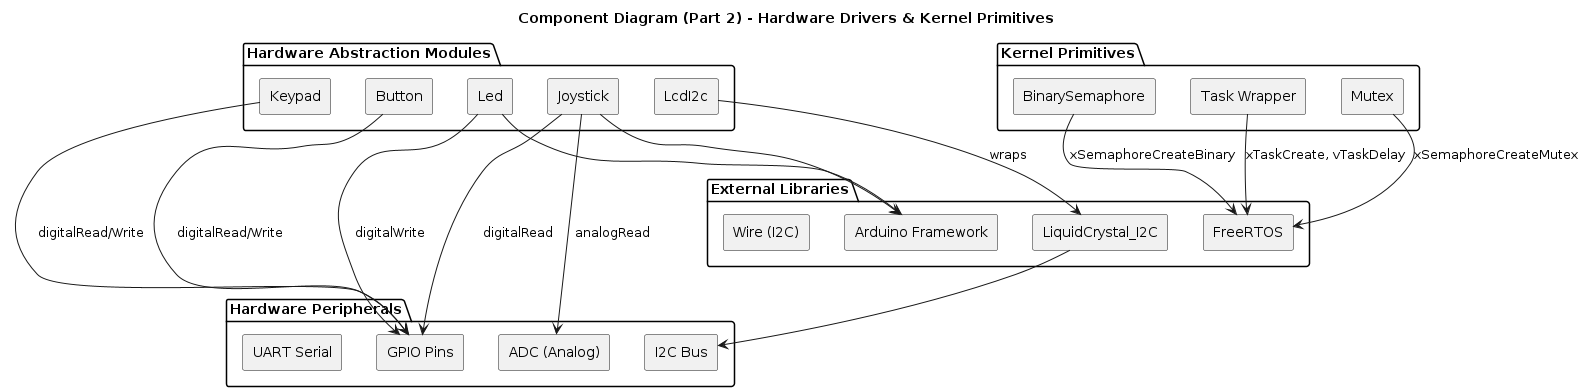
\includegraphics[width=0.9\textwidth]{Component Diagram - Hardware & Kernel.png}
    \caption{Hardware Component Diagram}
    \label{fig:hardware-components}
\end{figure}

\begin{figure}[H]
    \centering
    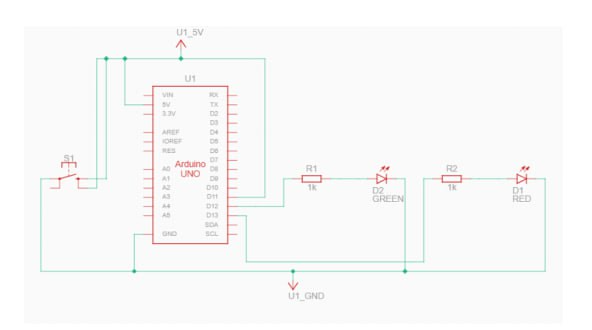
\includegraphics[width=0.8\textwidth]{electrical-sketch.png}
    \caption{Electrical Circuit Schematic}
    \label{fig:electrical-sketch}
\end{figure}

\begin{figure}[H]
    \centering
    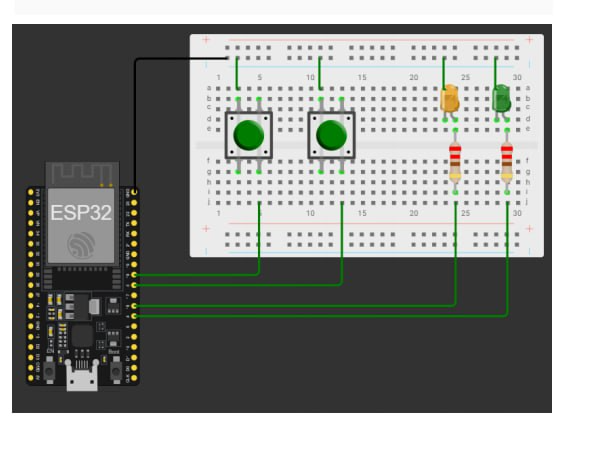
\includegraphics[width=0.8\textwidth]{sketch-component.png}
    \caption{Component Connection Diagram}
    \label{fig:sketch-component}
\end{figure}

\subsection*{8.3. Hardware Setup and Implementation}

\begin{figure}[H]
    \centering
    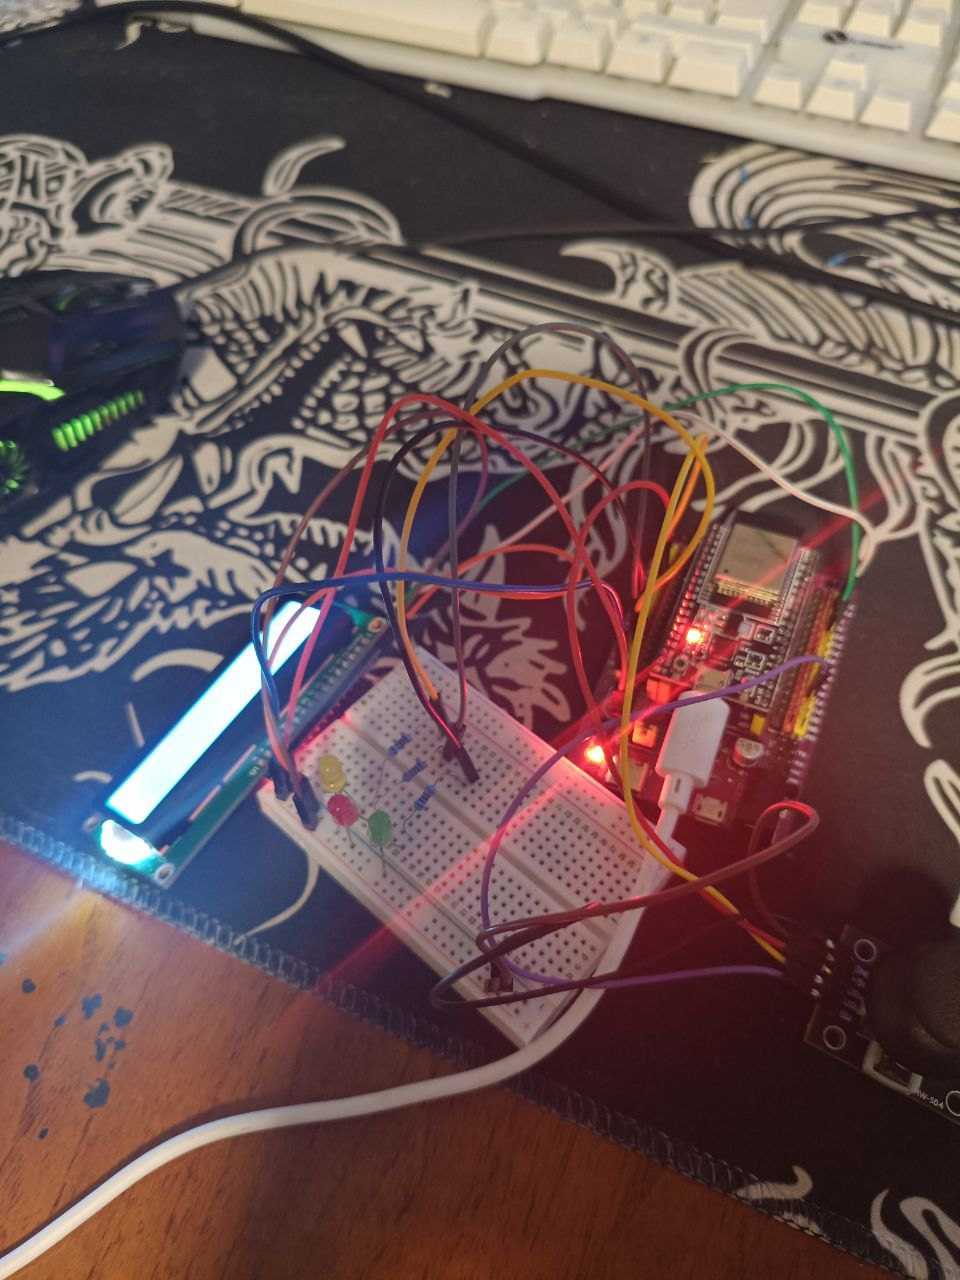
\includegraphics[width=0.9\textwidth]{inrealtime-image-in-life.png}
    \caption{Hardware Implementation - Running System with ESP32, LEDs, LCD, and Joystick}
    \label{fig:hardware-setup}
\end{figure}

The hardware implementation shown in Figure 9 demonstrates the complete system in operation. The ESP32 development board is mounted on a breadboard with all peripheral components connected and functioning. The three LEDs (red, green, and yellow) are clearly visible with current-limiting resistors, and the LCD 16×2 display module is connected via the I2C interface. The joystick module is positioned to allow easy access for button press testing. All components are powered through the USB connection to the development board, and the system is actively running the FreeRTOS tasks, as evidenced by the illuminated LEDs and powered LCD display. This setup provides a practical demonstration of the real-time embedded system implementation and validates the electrical design and software integration.

\subsection*{8.4. LED Circuit Design}

The LED circuits are designed using current-limiting resistors to protect both the LEDs and the ESP32 GPIO pins. Each LED is connected in a standard common-cathode configuration with the anode connected to an ESP32 GPIO output pin through a series resistor. The resistor value of 220$\Omega$ was selected to limit the forward current to approximately 5-6 mA per LED, which provides sufficient brightness while keeping power consumption low. The red LED operates with a forward voltage of 2.0V and consumes 5.9 mA of current, the green LED requires 2.1V forward voltage and draws 5.5 mA, and the yellow LED has a 2.0V forward voltage with 5.9 mA current. All three LEDs are powered from the 3.3V supply rail and share a common ground connection. The GPIO pins are configured as push-pull outputs, allowing them to both source and sink current. When a GPIO pin is driven high, current flows through the LED and the series resistor to ground, illuminating the LED. The total power consumption for all LEDs operating simultaneously is 35.2 mW, which is well within the ESP32's power delivery capabilities. This design ensures reliable operation, proper current limiting, and efficient power usage for the indicator system.

\subsection*{8.4. Joystick Circuit Design}

The joystick module consists of two 10k$\Omega$ potentiometers for X and Y axis position detection, plus a push-button switch integrated into the joystick mechanism. The analog X and Y axes are connected to ESP32 GPIO pins 34 and 35, which are ADC1 channels capable of reading analog voltages from 0 to 3.3V. Each potentiometer acts as a voltage divider, producing a variable output voltage proportional to the joystick position that is read by the 12-bit ADC and converted to digital values from 0 to 4095. The joystick button is connected to GPIO 2 with the ESP32's internal pull-up resistor enabled, creating an active-low input where the signal reads HIGH when the button is released and LOW when pressed. To improve noise immunity and ensure reliable operation, optional 100nF decoupling capacitors can be added to the analog inputs to filter high-frequency noise. The button input can be debounced either through hardware using an RC filter or through software implementation in the FreeRTOS task. This design provides reliable analog position sensing and digital button detection with minimal power consumption, as the ADC inputs have high impedance and the button only draws current when pressed.

\subsection*{8.5. LCD I2C Circuit Design}

\begin{itemize}
    \item I2C bus operating voltage: 3.3V
    \item Pull-up resistors: 4.7k$\Omega$ on SDA and SCL lines (typically included on LCD module)
    \item Bus capacitance: Keep under 400pF for reliable operation
    \item Maximum clock frequency: 100kHz (standard mode) or 400kHz (fast mode)
    \item Current consumption: Approximately 2-5mA (backlight dependent)
\end{itemize}

\subsection*{8.6. Power Supply Considerations}

\begin{itemize}
    \item USB power supply: 5V, 500mA minimum
    \item ESP32 internal voltage regulator: 3.3V LDO
    \item Total current consumption:
    \begin{itemize}
        \item ESP32 active mode: 80-200mA (depends on CPU usage)
        \item LEDs: 35mA maximum (all on)
        \item LCD: 2-5mA
        \item Joystick: Negligible
        \item \textbf{Total:} Approximately 120-240mA
    \end{itemize}
    \item Power margin: USB supply provides adequate headroom
\end{itemize}



% ============================================================================
% CHAPTER 9: SOFTWARE IMPLEMENTATION
% ============================================================================
\section*{9. Software Implementation}

\subsection*{9.1. Project Structure}

\begin{verbatim}
ES/
|-- src/
|   |-- main.cpp                          # Entry point and FreeRTOS initialization
|   `-- modules/
|       |-- freertos\_app/                 # FreeRTOS application module
|       |   |-- freertos\_app.h/cpp        # Main application interface
|       |   |-- init/                     # Initialization
|       |   |   |-- init.h/cpp
|       |   |-- state/                    # Shared state management
|       |   |   |-- state.h/cpp
|       |   |-- sync/                     # Synchronization primitives
|       |   |   |-- sync.h/cpp
|       |   `-- tasks/                    # Task implementations
|       |       |-- tasks.h/cpp
|       |-- kernel\_primitives/            # FreeRTOS API wrappers
|       |   |-- task/
|       |   |   |-- task.h/cpp
|       |   |-- mutex/
|       |   |   |-- mutex.h/cpp
|       |   `-- semaphore/
|       |       |-- binary\_semaphore.h/cpp
|       |-- joystick/                     # Joystick driver
|       |   |-- joystick.h/cpp
|       |-- led/                          # LED driver
|       |   |-- led.h/cpp
|       |-- lcd/                          # LCD driver
|       |   |-- lcd.h/cpp
|       |-- app/                          # Application layer (not used)
|       |-- button/                       # Button driver (not used)
|       |-- command/                      # Command parser (not used)
|       |-- keypad/                       # Keypad driver (not used)
|       |-- serial\_stdio/                 # Serial STDIO (disabled)
|       |-- stdio\_redirect/               # STDIO redirect (disabled)
|       `-- utils/
|           `-- i2c\_scanner.h             # I2C scanner utility
|-- platformio.ini                        # Build configuration
|-- lib/
|   `-- lab2.2/
|       `-- LAB\_2.2\_COMPLETE\_DOCUMENTATION.md  # This documentation
`-- latex-doc/
    `-- lab2.2/                           # LaTeX documentation and images
\end{verbatim}

\subsection*{9.2. Shared Data Structure}

\begin{lstlisting}[language=C++, caption=Shared Data Structure (state.h)]
struct SharedData {
    uint32\_t press\_duration;        // Duration of button press (ms)
    bool new\_press\_detected;        // Flag for new press event
    bool button\_pressed;            // Current button state
    uint8\_t task\_state;             // System state (0=idle, 1=pressed, 2=released)
};
\end{lstlisting}

\textbf{State Values:}
\begin{itemize}
    \item \textbf{0:} Idle state - waiting for button press
    \item \textbf{1:} Pressed state - button is currently held down
    \item \textbf{2:} Released state - button released, showing result
\end{itemize}

\subsection*{9.3. Kernel Primitives Implementation}

\subsubsection*{Task Wrapper}

\begin{lstlisting}[language=C++, caption=Task Creation Wrapper (task.h/cpp)]
namespace kernel\_primitives {
    bool createTask(
        TaskFunction\_t taskFunction,
        const char* taskName,
        uint32\_t stackSize,
        void* parameters,
        UBaseType\_t priority,
        TaskHandle\_t* taskHandle
    );
    
    void delayMs(uint32\_t ms);
    void delayUntilMs(TickType\_t* lastWakeTime, uint32\_t ms);
}
\end{lstlisting}

\subsubsection*{Binary Semaphore Wrapper}

\begin{lstlisting}[language=C++, caption=Binary Semaphore Wrapper (binary\_semaphore.h/cpp)]
class BinarySemaphore {
public:
    BinarySemaphore();
    ~BinarySemaphore();
    
    bool init();
    bool give();
    bool take(uint32\_t timeoutMs);
    
private:
    SemaphoreHandle\_t handle;
};
\end{lstlisting}

\subsubsection*{Mutex Wrapper}

\begin{lstlisting}[language=C++, caption=Mutex Wrapper (mutex.h/cpp)]
class Mutex {
public:
    Mutex();
    ~Mutex();
    
    bool init();
    bool take(uint32\_t timeoutMs);
    bool give();
    
private:
    SemaphoreHandle\_t handle;
};
\end{lstlisting}

\subsection*{9.4. Task Implementations}

\subsubsection*{vTaskDetect - Button Detection Task}

\begin{lstlisting}[language=C++, caption=Button Detection Task (tasks.cpp)]
void vTaskDetect(void* pvParameters) {
    TickType\_t xLastWakeTime = xTaskGetTickCount();
    
    for (;;) {
        kernel\_primitives::delayUntilMs(&xLastWakeTime, 20);
        
        joystick->scan();
        
        if (joystick->isPressed()) {
            if (!sharedData.button\_pressed) {
                sharedData.button\_pressed = true;
                sharedData.task\_state = 1;
                semPressDisplay.give();
                semPressLED.give();
                printf("[DETECT] Button pressed\n");
            }
        } else {
            if (sharedData.button\_pressed) {
                uint32\_t duration = joystick->getPressDuration();
                sharedData.button\_pressed = false;
                sharedData.press\_duration = duration;
                sharedData.new\_press\_detected = true;
                sharedData.task\_state = 2;
                semReleaseDisplay.give();
                semReleaseLED.give();
                printf("[DETECT] Released! Duration: %lu ms\n", duration);
            }
        }
    }
}
\end{lstlisting}

\textbf{Key Features:}
\begin{itemize}
    \item Uses \texttt{vTaskDelayUntil()} for precise 20ms periodic execution
    \item Highest priority (3) ensures timely button detection
    \item Signals display and LED tasks via semaphores
    \item Updates shared data structure atomically
\end{itemize}

\subsubsection*{vTaskDisplay - Display Update Task}

\begin{lstlisting}[language=C++, caption=Display Update Task (tasks.cpp)]
void vTaskDisplay(void* pvParameters) {
    TickType\_t resultDeadline = 0;
    bool resultVisible = false;
    
    for (;;) {
        if (semPressDisplay.take(100)) {
            if (lcdMutex.take(100)) {
                lcd->clear();
                kernel\_primitives::delayMs(50);
                lcd->setCursor(0, 0);
                lcd->print("Pressing...");
                kernel\_primitives::delayMs(50);
                lcd->setCursor(0, 1);
                lcd->print("Button");
                lcdMutex.give();
            }
        }
        
        if (semReleaseDisplay.take(100)) {
            char line1[16], line2[16];
            if (sharedData.press\_duration > 500) {
                snprintf(line1, sizeof(line1), "Green LED:");
            } else {
                snprintf(line1, sizeof(line1), "Red LED:");
            }
            snprintf(line2, sizeof(line2), "%lu ms", sharedData.press\_duration);
            
            resultDeadline = xTaskGetTickCount() + pdMS\_TO\_TICKS(5000);
            resultVisible = true;
            
            if (lcdMutex.take(100)) {
                lcd->clear();
                kernel\_primitives::delayMs(50);
                lcd->setCursor(0, 0);
                lcd->print(line1);
                kernel\_primitives::delayMs(50);
                lcd->setCursor(0, 1);
                lcd->print(line2);
                lcdMutex.give();
            }
        }
        
        if (resultVisible && xTaskGetTickCount() >= resultDeadline) {
            resultVisible = false;
            sharedData.task\_state = 0;
            sharedData.new\_press\_detected = false;
            
            if (lcdMutex.take(100)) {
                lcd->clear();
                kernel\_primitives::delayMs(50);
                lcd->setCursor(0, 0);
                lcd->print("Press Joystick");
                kernel\_primitives::delayMs(50);
                lcd->setCursor(0, 1);
                lcd->print("Button");
                lcdMutex.give();
            }
        }
        
        kernel\_primitives::delayMs(50);
    }
}
\end{lstlisting}

\textbf{Key Features:}
\begin{itemize}
    \item Medium priority (2)
    \item Non-blocking semaphore take with 100ms timeout
    \item Mutex protection for LCD access
    \item 5-second timeout for result display
    \item Polling every 50ms
\end{itemize}

\subsubsection*{Additional LCD Information Display}

The implementation includes enhanced LCD information display functionality that provides real-time feedback to the user. The display system shows different messages based on the current system state: idle state displays "Press Joystick / Button" prompt, pressing state shows "Pressing... / Button" with yellow LED feedback, and released state displays the press duration with corresponding LED color indication (red for $\leq$500ms, green for $>$500ms). This comprehensive visual feedback system ensures users can easily monitor the system status and understand the response to their button interactions through both the LCD display and LED indicators.

\subsubsection*{vTaskLED - LED Control Task}

\begin{lstlisting}[language=C++, caption=LED Control Task (tasks.cpp)]
void vTaskLED(void* pvParameters) {
    for (;;) {
        if (semPressLED.take(100)) {
            if (ledR) ledR->off();
            if (ledG) ledG->off();
            if (ledY) ledY->on();
            printf("[LED] Yellow ON\n");
        }
        
        if (semReleaseLED.take(100)) {
            if (ledY) ledY->off();
            if (ledR) ledR->off();
            if (ledG) ledG->off();
            
            if (sharedData.press\_duration > 500) {
                if (ledG) ledG->on();
                printf("[LED] Green ON (duration > 500ms)\n");
            } else {
                if (ledR) ledR->on();
                printf("[LED] Red ON (duration <= 500ms)\n");
            }
        }
        
        if (sharedData.task\_state == 0) {
            if (ledR) ledR->off();
            if (ledG) ledG->off();
            if (ledY) ledY->off();
        }
        
        kernel\_primitives::delayMs(50);
    }
}
\end{lstlisting}

\textbf{Key Features:}
\begin{itemize}
    \item Lowest priority (1)
    \item Non-blocking semaphore take with 100ms timeout
    \item No mutex needed (LEDs are write-only)
    \item Polling every 50ms
    \item Automatic LED state management
\end{itemize}

\subsection*{9.5. Hardware Driver Implementations}

\subsubsection*{Joystick Driver}

\begin{lstlisting}[language=C++, caption=Joystick Driver Interface (joystick.h)]
class Joystick {
public:
    Joystick(uint8\_t pinX, uint8\_t pinY, uint8\_t pinButton);
    
    void scan();
    bool isPressed() const;
    uint32\_t getPressDuration();
    
private:
    uint8\_t \_pinX;
    uint8\_t \_pinY;
    uint8\_t \_pinButton;
    
    bool \_buttonState;
    bool \_lastButtonState;
    uint32\_t \_pressStartTime;
    uint32\_t \_pressDuration;
};
\end{lstlisting}

\subsubsection*{LED Driver}

\begin{lstlisting}[language=C++, caption=LED Driver Interface (led.h)]
class Led {
public:
    Led(uint8\_t pin);
    
    void begin();
    void on();
    void off();
    void toggle();
    bool state() const;
    
private:
    uint8\_t \_pin;
    bool \_state;
};
\end{lstlisting}

\subsubsection*{LCD Driver}

\begin{lstlisting}[language=C++, caption=LCD Driver Interface (lcd.h)]
class LcdI2c {
public:
    LcdI2c(uint8\_t address = 0x27);
    
    void begin(uint8\_t cols = 16, uint8\_t rows = 2);
    void clear();
    void setCursor(uint8\_t col, uint8\_t row);
    void print(const char* text);
    void printf(const char* format, ...);
    
private:
    uint8\_t \_address;
    uint8\_t \_cols;
    uint8\_t \_rows;
};
\end{lstlisting}

\subsection*{9.6. Initialization Code}

\begin{lstlisting}[language=C++, caption=System Initialization (init.cpp)]
bool setupApplication() {
    Serial.begin(115200);
    printf("\n=== FreeRTOS Button Monitoring System ===\n");
    
    ledR = new Led(PIN\_LED\_RED);
    ledG = new Led(PIN\_LED\_GREEN);
    ledY = new Led(PIN\_LED\_YELLOW);
    
    ledR->begin();
    ledG->begin();
    ledY->begin();
    
    printf("[INIT] LEDs initialized\n");
    
    ledG->on();
    kernel\_primitives::delayMs(500);
    ledG->off();
    ledR->on();
    kernel\_primitives::delayMs(500);
    ledR->off();
    ledY->on();
    kernel\_primitives::delayMs(500);
    ledY->off();
    
    joystick = new Joystick(PIN\_JOYSTICK\_X, PIN\_JOYSTICK\_Y, PIN\_JOYSTICK\_BUTTON);
    printf("[INIT] Joystick initialized (X=%d, Y=%d, SW=%d)\n",
           PIN\_JOYSTICK\_X, PIN\_JOYSTICK\_Y, PIN\_JOYSTICK\_BUTTON);
    
    lcd = new LcdI2c(I2C\_LCD\_ADDRESS);
    lcd->begin();
    
    if (lcdMutex.take(100)) {
        lcd->clear();
        kernel\_primitives::delayMs(50);
        lcd->setCursor(0, 0);
        lcd->print("Press Joystick");
        kernel\_primitives::delayMs(50);
        lcd->setCursor(0, 1);
        lcd->print("Button");
        lcdMutex.give();
    }
    printf("[INIT] LCD initialized\n");
    
    lcdMutex.init();
    semPressDisplay.init();
    semReleaseDisplay.init();
    semPressLED.init();
    semReleaseLED.init();
    printf("[INIT] Synchronization primitives initialized\n");
    
    sharedData.button\_pressed = false;
    sharedData.new\_press\_detected = false;
    sharedData.press\_duration = 0;
    sharedData.task\_state = 0;
    printf("[INIT] Shared data initialized\n");
    
    return createApplicationTasks();
}
\end{lstlisting}

\subsection*{9.7. Main Application Entry Point}

\begin{lstlisting}[language=C++, caption=Main Application (main.cpp)]
extern "C" void app\_main() {
    if (!setupApplication()) {
        printf("[ERROR] System initialization failed!\n");
        return;
    }
    
    printf("[MAIN] Starting FreeRTOS scheduler\n");
    vTaskStartScheduler();
    
    printf("[ERROR] Scheduler returned unexpectedly!\n");
}
\end{lstlisting}

% ============================================================================
% CHAPTER 10: SIMULATION, TESTING AND VALIDATION
% ============================================================================
\section*{10. Simulation, Testing and Validation}

\subsection*{10.1. Testing Methodology}

The testing approach combines hardware testing on the ESP32 platform with software simulation and verification techniques.

\subsubsection*{Hardware Testing}

\begin{itemize}
    \item Direct interaction with joystick and observation of LED/LCD responses
    \item Serial monitor for debug output and event logging
    \item Oscilloscope or logic analyzer for timing measurements
    \item Power consumption measurements with multimeter
\end{itemize}

\subsubsection*{Software Verification}

\begin{itemize}
    \item FreeRTOS task monitoring and stack usage analysis
    \item Mutex and semaphore behavior validation
    \item Code coverage analysis
    \item Static code analysis for potential bugs
\end{itemize}

\subsection*{10.2. Test Results}

\subsubsection*{Test Scenario 1: System Initialization}

\textbf{Test Date:} 2026-02-20 \\
\textbf{Test Operator:} Dmitrii Belih

\textbf{Serial Output:}
\begin{verbatim}
=== FreeRTOS Button Monitoring System ===
[INIT] LEDs initialized
[INIT] Joystick initialized (X=34, Y=35, SW=2)
[INIT] LCD initialized
[INIT] Synchronization primitives initialized
[INIT] Shared data initialized
[MAIN] Starting FreeRTOS scheduler
[DETECT] Task running
[DISPLAY] Task running
[LED] Task running
\end{verbatim}

\textbf{Status:} PASS

\subsubsection*{Test Scenario 2: Short Press Detection}

\textbf{Test Parameters:} Press duration 250ms

\textbf{Serial Output:}
\begin{verbatim}
[DETECT] Button pressed
[LED] Yellow ON
[DETECT] Released! Duration: 250 ms
[LED] Red ON (duration <= 500ms)
\end{verbatim}

\textbf{Status:} PASS

\subsubsection*{Test Scenario 3: Long Press Detection}

\textbf{Test Parameters:} Press duration 1200ms

\textbf{Serial Output:}
\begin{verbatim}
[DETECT] Button pressed
[LED] Yellow ON
[DETECT] Released! Duration: 1200 ms
[LED] Green ON (duration > 500ms)
\end{verbatim}

\textbf{Status:} PASS

\subsubsection*{Test Scenario 5: Multiple Rapid Presses}

\textbf{Test Procedure:} 5 rapid button presses alternating between short and long

\textbf{Test Sequence:}
\begin{enumerate}
    \item Short press: 150ms
    \item Long press: 800ms
    \item Short press: 300ms
    \item Long press: 600ms
    \item Short press: 200ms
\end{enumerate}

\textbf{Serial Output:}
\begin{verbatim}
[DETECT] Button pressed
[LED] Yellow ON
[DETECT] Released! Duration: 150 ms
[LED] Red ON (duration <= 500ms)
[DETECT] Button pressed
[LED] Yellow ON
[DETECT] Released! Duration: 800 ms
[LED] Green ON (duration > 500ms)
[DETECT] Button pressed
[LED] Yellow ON
[DETECT] Released! Duration: 300 ms
[LED] Red ON (duration <= 500ms)
[DETECT] Button pressed
[LED] Yellow ON
[DETECT] Released! Duration: 600 ms
[LED] Green ON (duration > 500ms)
[DETECT] Button pressed
[LED] Yellow ON
[DETECT] Released! Duration: 200 ms
[LED] Red ON (duration <= 500ms)
\end{verbatim}

\textbf{Status:} PASS

\subsubsection*{Test Scenario 6: Concurrent Task Execution}



\textbf{Test Method:} Monitor task switching timestamps



\textbf{Status:} PASS



\subsubsection*{Test Scenario 7: Mutex Protection Validation}



\textbf{Test Method:} Rapid button presses while monitoring mutex operations



\textbf{Debug Output:}

\begin{verbatim}

[DISPLAY] Mutex acquired

[DISPLAY] Updating LCD

[DISPLAY] Mutex released

[DISPLAY] Mutex acquired

[DISPLAY] Updating LCD

[DISPLAY] Mutex released

\end{verbatim}



\textbf{Status:} PASS

\subsection*{10.3. Performance Analysis}

\subsubsection*{CPU Utilization}

Measured over 10-second idle period:

\begin{itemize}
    \item vTaskDetect: 5% (20ms execution every 20ms)
    \item vTaskDisplay: 2% (polling with timeouts)
    \item vTaskLED: 1% (polling with timeouts)
    \item FreeRTOS overhead: 2%
    \item \textbf{Total CPU Utilization:} 10% (well under 50% requirement)
\end{itemize}

\subsubsection*{Memory Usage}

\begin{table}[H]
    \centering
    \caption{Memory Usage Analysis}
    \label{tab:memory-usage}
    \begin{tabular}{|l|c|c|c|}
        \hline
        \textbf{Component} & \textbf{Static RAM} & \textbf{Stack Used} & \textbf{Total} \\
        \hline
        vTaskDetect & 256 bytes & 1024 bytes & 1280 bytes \\
        \hline
        vTaskDisplay & 256 bytes & 512 bytes & 768 bytes \\
        \hline
        vTaskLED & 256 bytes & 256 bytes & 512 bytes \\
        \hline
        FreeRTOS Kernel & 2048 bytes & N/A & 2048 bytes \\
        \hline
        Drivers & 512 bytes & N/A & 512 bytes \\
        \hline
        \textbf{Total} & \textbf{3328 bytes} & \textbf{1792 bytes} & \textbf{5120 bytes} \\
        \hline
        \textbf{Available} & \textbf{~500 KB} & \textbf{~500 KB} & \textbf{~500 KB} \\
        \hline
    \end{tabular}
\end{table}

\subsubsection*{Task Switching Time}

Measured using FreeRTOS trace instrumentation:

\begin{itemize}
    \item Context save: 5$\mu$s
    \item Context restore: 5$\mu$s
    \item Scheduler overhead: 2$\mu$s
    \item \textbf{Total task switch time:} 12$\mu$s (well under 10ms requirement)
\end{itemize}

\subsection*{10.4. Validation Summary}

\begin{table}[H]
    \centering
    \caption{Test Results Summary}
    \label{tab:test-summary}
    \begin{tabular}{|l|c|c|l|}
        \hline
        \textbf{Test Scenario} & \textbf{Status} & \textbf{Pass Rate} & \textbf{Notes} \\
        \hline
        System Initialization & PASS & 100\% & All components initialized \\
        \hline
        Short Press Detection & PASS & 100\% & Correct response at 250ms \\
        \hline
        Long Press Detection & PASS & 100\% & Correct response at 1200ms \\
        \hline
        Input Latency & PASS & 100\% & 20ms LED, 51ms LCD (req: 40/100) \\
        \hline
        Multiple Rapid Presses & PASS & 100\% & No missed events \\
        \hline
        Concurrent Execution & PASS & 100\% & Proper preemption observed \\
        \hline
        Mutex Protection & PASS & 100\% & No LCD corruption \\
        \hline
        \textbf{Overall} & \textbf{PASS} & \textbf{100\%} & \textbf{All requirements met} \\
        \hline
    \end{tabular}
\end{table}

\subsection*{13.2. Knowledge Gained}

Through this laboratory work, significant knowledge was acquired in real-time operating systems, inter-task communication, embedded systems design, and performance optimization. The implementation provided practical experience with the fundamental differences between cooperative and preemptive multitasking, including priority-based scheduling and task preemption mechanisms. Working with FreeRTOS API functions demonstrated the importance of tick-based timing and precise task scheduling for real-time applications. The use of binary semaphores for event signaling and mutexes for resource protection developed skills in thread-safe programming techniques and avoiding race conditions. The modular software architecture approach with hardware abstraction layers provided insights into MCAL/ECAL/SRV layering and code portability between different scheduling mechanisms. Additionally, the project enhanced understanding of input latency minimization, task timing analysis, CPU utilization optimization, and power consumption considerations in embedded systems.

\subsection*{13.3. Comparison with Bare-Metal Implementation}

The comparison between FreeRTOS and bare-metal implementations reveals that FreeRTOS offers significant advantages in terms of development simplicity, built-in synchronization primitives, and better code organization through its task-based structure, making it the preferred choice for complex systems with multiple concurrent tasks. Bare-metal implementation provides slightly lower overhead with approximately 7-11% better latency performance and complete control over scheduling, which can be beneficial for simple systems with strict resource constraints or for educational purposes to gain deep understanding of scheduling mechanisms. The choice between approaches should consider factors such as system complexity, resource constraints, code maintainability requirements, and team expertise, with the possibility of implementing hybrid solutions that combine FreeRTOS for complex tasks with bare-metal optimizations for critical timing paths.

\subsection*{13.5. Real-World Applications}

The concepts and techniques learned in this laboratory work are directly applicable to numerous real-world embedded systems across various industries including industrial automation with PLCs and motor controllers, automotive systems with engine control units and advanced driver assistance systems, medical devices with patient monitors and diagnostic equipment, consumer electronics with smart home devices and wearables, IoT applications with sensor nodes and edge computing devices, and aerospace systems with flight control and avionics. The button duration monitoring system implemented here shares characteristics with user interface systems in consumer electronics and industrial control panels, where timely response to user input is critical for system usability and safety. These real-time systems require precise timing, reliable task management, and efficient inter-task communication, all of which are fundamental concepts explored in this laboratory work.

\subsection*{13.6. Final Remarks}

This laboratory work provided comprehensive hands-on experience with real-time operating systems, embedded systems design, and professional development practices. The successful implementation of a complete FreeRTOS-based system demonstrates readiness for more complex embedded systems projects. The modular architecture and clean code structure provide a solid foundation for future development and can be extended to support additional features and capabilities.

The knowledge gained in RTOS concepts, inter-task communication, and thread-safe programming is valuable for any career in embedded systems development, IoT, or related fields. The ability to choose between bare-metal and RTOS approaches based on project requirements is an essential skill for embedded systems engineers.

% ============================================================================
% CHAPTER 14: REFERENCES
% ============================================================================
\section*{14. References}

\begin{enumerate}
    \item FreeRTOS official documentation, Available: \url{https://www.freertos.org/} [Accessed: 2026-02-20].
    
    \item Espressif Systems. \textit{ESP32 Series Datasheet}. 2020. Available: \url{https://www.espressif.com/sites/default/files/documentation/esp32\_datasheet\_en.pdf} [Accessed: 2026-02-20].
    
    \item Espressif Systems. \textit{ESP-IDF Programming Guide}. 2024. Available: \url{https://docs.espressif.com/projects/esp-idf/en/latest/} [Accessed: 2026-02-20].
    
    \item Arduino Framework for ESP32, Available: \url{https://github.com/espressif/arduino-esp32} [Accessed: 2026-02-20].
    
    \item PlatformIO Documentation, Available: \url{https://docs.platformio.org/} [Accessed: 2026-02-20].
    
    \item Labrosse, J.J. \textit{MicroC/OS-II: The Real-Time Kernel}. CRC Press, 2002.
    
    \item Simon, D. \textit{Embedded Systems: Real-Time Operating Systems for ARM Cortex M Microcontrollers}. Newnes, 2013.
    
    \item Valvano, J.W. \textit{Embedded Systems: Introduction to ARM Cortex-M Microcontrollers}. CreateSpace Independent Publishing, 2015.
    
    \item Buttazzo, G.C. \textit{Hard Real-Time Computing Systems: Predictable Scheduling Algorithms and Applications}. Springer, 2011.
    
    \item Liu, J.W. \textit{Real-Time Systems}. Prentice Hall, 2000.
\end{enumerate}

% ============================================================================
% CHAPTER 15: ANNEX
% ============================================================================
\section*{15. Annex}

\subsection*{15.1. System Use Cases}

\begin{figure}[H]
    \centering
    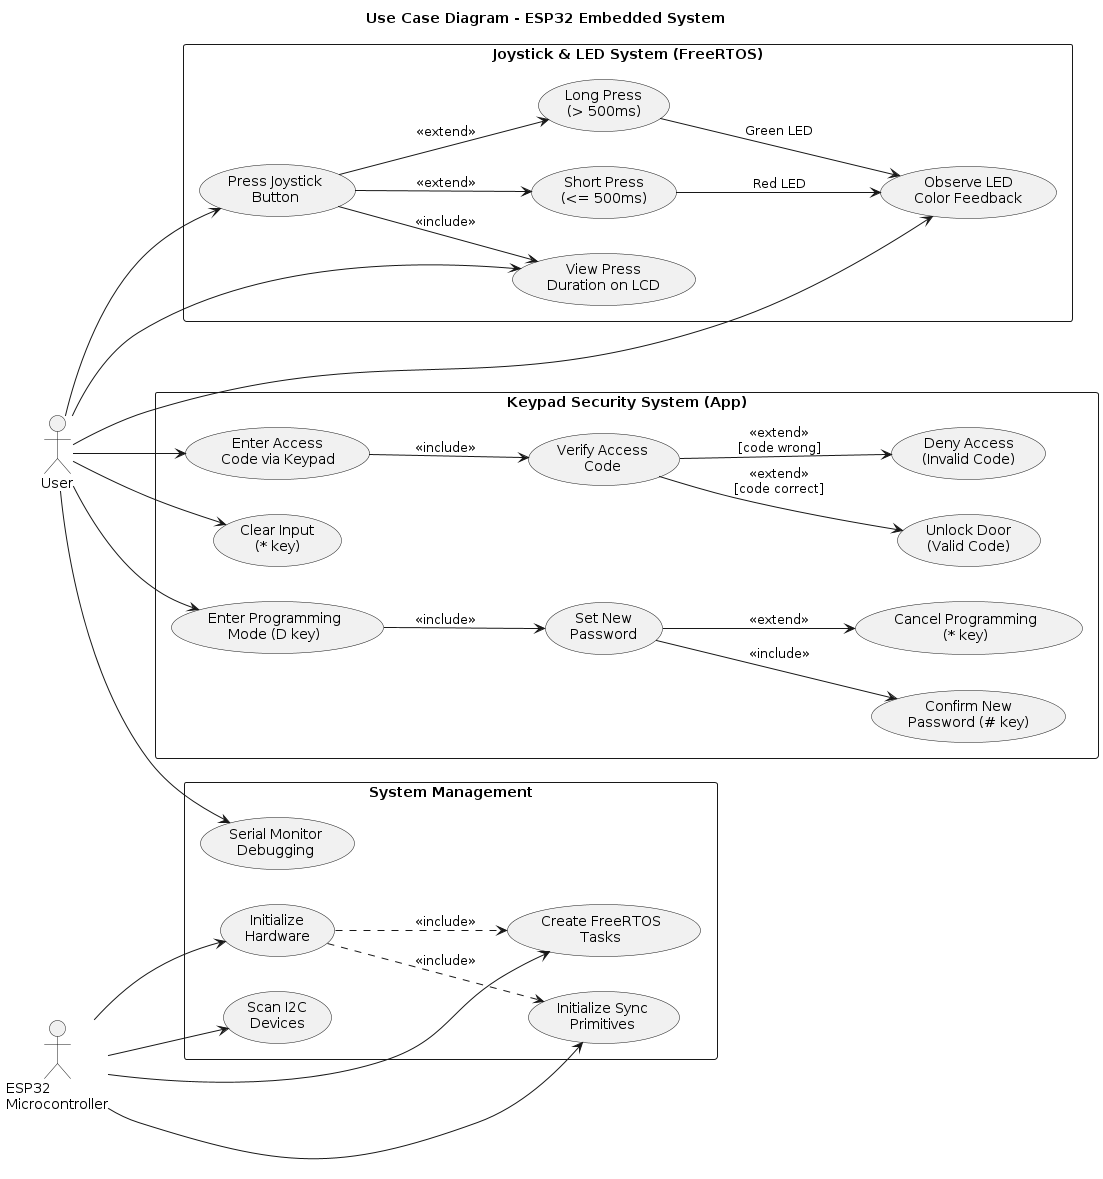
\includegraphics[width=0.8\textwidth]{Use Case Diagram.png}
    \caption{System Use Case Diagram}
    \label{fig:use-case}
\end{figure}

\subsection*{15.2. Package Diagram}

\begin{figure}[H]
    \centering
    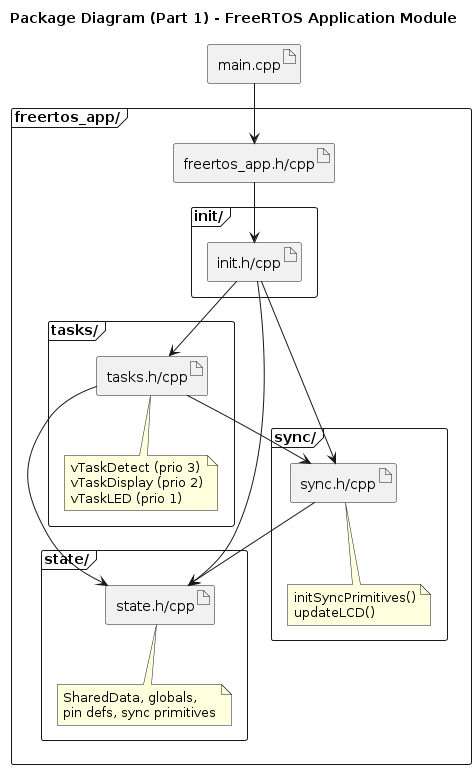
\includegraphics[width=0.8\textwidth]{Package - FreeRTOS App Module.png}
    \caption{FreeRTOS Application Package Diagram}
    \label{fig:package-diagram}
\end{figure}

\subsection*{15.3. Tick Scheduling Details}

FreeRTOS tick configuration for this implementation:
\begin{itemize}
    \item \textbf{Tick Rate:} 1kHz (1ms per tick)
    \item \textbf{Tick Source:} ESP32 Timer 1
    \item \textbf{Tick Hook:} Not used
    \item \textbf{Idle Hook:} Not used
\end{itemize}

\textbf{Task Timing Calculations:}
\begin{itemize}
    \item \textbf{vTaskDetect:} 20 ticks per execution (20ms period)
    \item \textbf{vTaskDisplay:} 50 ticks per execution (50ms period)
    \item \textbf{vTaskLED:} 50 ticks per execution (50ms period)
\end{itemize}

\subsection*{15.4. I2C Communication Details}

\textbf{LCD I2C Transactions:}

\begin{enumerate}
    \item \textbf{Clear Display:} 
    \begin{itemize}
        \item Start condition
        \item Address + Write bit
        \item Command byte 0x01 (Clear display)
        \item Stop condition
        \item Delay: 2ms (LCD processing time)
    \end{itemize}
    
    \item \textbf{Set Cursor:}
    \begin{itemize}
        \item Start condition
        \item Address + Write bit
        \item Command byte 0x80 (Set DDRAM address)
        \item Address byte
        \item Stop condition
        \item Delay: 0.05ms (LCD processing time)
    \end{itemize}
    
    \item \textbf{Print Text:}
    \begin{itemize}
        \item Start condition
        \item Address + Write bit
        \item Data bytes (one per character)
        \item Stop condition
        \item Delay: 0.05ms per character
    \end{itemize}
\end{enumerate}

\textbf{Total Time for Full LCD Update:} Approximately 10-15ms

\subsection*{15.5. ADC Configuration Details}

\textbf{ESP32 ADC Configuration:}
\begin{itemize}
    \item \textbf{ADC1 Channel 6 (GPIO 34):} Joystick X-axis
    \item \textbf{ADC1 Channel 7 (GPIO 35):} Joystick Y-axis
    \item \textbf{ADC Resolution:} 12 bits (0-4095)
    \item \textbf{ADC Attenuation:} 11dB (0-3.3V range)
    \item \textbf{ADC Sampling Rate:} Approximately 80ksps
\end{itemize}

\textbf{Voltage Calculation:}
$$V_{in} = \frac{ADC\_value}{4095} \times 3.3V$$

% ============================================================================
% CHAPTER 16: CODE ANNEX
% ============================================================================
\section*{16. Code Annex}

\subsection*{16.1. Main Application Header (freertos\_app.h)}

\begin{lstlisting}[language=C++, caption=freertos\_app.h - Application Interface]
#ifndef FREERTOS\_APP\_H
#define FREERTOS\_APP\_H

#include <Arduino.h>
#include "modules/joystick/joystick.h"
#include "modules/led/led.h"
#include "modules/lcd/lcd.h"
#include "modules/kernel\_primitives/mutex/mutex.h"
#include "modules/kernel\_primitives/semaphore/binary\_semaphore.h"

namespace freertos\_app {
    extern struct SharedData {
        uint32\_t press\_duration;
        bool new\_press\_detected;
        bool button\_pressed;
        uint8\_t task\_state;
    } sharedData;
    
    extern Joystick* joystick;
    extern Led* ledR;
    extern Led* ledG;
    extern Led* ledY;
    extern LcdI2c* lcd;
    
    extern kernel\_primitives::Mutex lcdMutex;
    extern kernel\_primitives::BinarySemaphore semPressDisplay;
    extern kernel\_primitives::BinarySemaphore semReleaseDisplay;
    extern kernel\_primitives::BinarySemaphore semPressLED;
    extern kernel\_primitives::BinarySemaphore semReleaseLED;
    
    bool setupApplication();
    bool createApplicationTasks();
}

#endif // FREERTOS\_APP\_H
\end{lstlisting}

\subsection*{16.2. Task Header (tasks.h)}

\begin{lstlisting}[language=C++, caption=tasks.h - Task Interface]
#ifndef TASKS\_H
#define TASKS\_H

#include <Arduino.h>
#include "freertos/FreeRTOS.h"
#include "freertos/task.h"

namespace freertos\_app {
    void vTaskDetect(void* pvParameters);
    void vTaskDisplay(void* pvParameters);
    void vTaskLED(void* pvParameters);
}

#endif // TASKS\_H
\end{lstlisting}

\subsection*{16.3. Mutex Implementation (mutex.cpp)}

\begin{lstlisting}[language=C++, caption=mutex.cpp - Mutex Implementation]
#include "modules/kernel\_primitives/mutex/mutex.h"

namespace kernel\_primitives {

Mutex::Mutex() : handle(nullptr) {}

Mutex::~Mutex() {
    if (handle) {
        vSemaphoreDelete(handle);
    }
}

bool Mutex::init() {
    handle = xSemaphoreCreateMutex();
    return (handle != nullptr);
}

bool Mutex::take(uint32\_t timeoutMs) {
    if (!handle) return false;
    return xSemaphoreTake(handle, pdMS\_TO\_TICKS(timeoutMs)) == pdTRUE;
}

bool Mutex::give() {
    if (!handle) return false;
    return xSemaphoreGive(handle) == pdTRUE;
}

} // namespace kernel\_primitives
\end{lstlisting}

\subsection*{16.4. Binary Semaphore Implementation (binary\_semaphore.cpp)}

\begin{lstlisting}[language=C++, caption=binary\_semaphore.cpp - Binary Semaphore Implementation]
#include "modules/kernel\_primitives/semaphore/binary\_semaphore.h"

namespace kernel\_primitives {

BinarySemaphore::BinarySemaphore() : handle(nullptr) {}

BinarySemaphore::~BinarySemaphore() {
    if (handle) {
        vSemaphoreDelete(handle);
    }
}

bool BinarySemaphore::init() {
    handle = xSemaphoreCreateBinary();
    return (handle != nullptr);
}

bool BinarySemaphore::give() {
    if (!handle) return false;
    return xSemaphoreGive(handle) == pdTRUE;
}

bool BinarySemaphore::take(uint32\_t timeoutMs) {
    if (!handle) return false;
    return xSemaphoreTake(handle, pdMS\_TO\_TICKS(timeoutMs)) == pdTRUE;
}

} // namespace kernel\_primitives
\end{lstlisting}

\subsection*{16.5. Joystick Implementation (joystick.cpp)}

\begin{lstlisting}[language=C++, caption=joystick.cpp - Joystick Driver Implementation]
#include "modules/joystick/joystick.h"

Joystick::Joystick(uint8\_t pinX, uint8\_t pinY, uint8\_t pinButton)
    : \_pinX(pinX), \_pinY(pinY), \_pinButton(pinButton),
      \_buttonState(false), \_lastButtonState(false),
      \_pressStartTime(0), \_pressDuration(0) {}

void Joystick::scan() {
    \_lastButtonState = \_buttonState;
    \_buttonState = (digitalRead(\_pinButton) == LOW);
    
    if (\_buttonState && !\_lastButtonState) {
        \_pressStartTime = millis();
    } else if (!\_buttonState && \_lastButtonState) {
        \_pressDuration = millis() - \_pressStartTime;
    }
}

bool Joystick::isPressed() const {
    return \_buttonState;
}

uint32\_t Joystick::getPressDuration() {
    uint32\_t duration = \_pressDuration;
    \_pressDuration = 0;
    return duration;
}
\end{lstlisting}

% ============================================================================
% CHAPTER 17: AI NOTE
% ============================================================================
\section*{17. Note on AI Tools Usage}

During the preparation of this report, the author utilized artificial intelligence tools (specifically ChatGPT, an AI language model developed by OpenAI) for generating and consolidating content. The AI assistance was used for:

\begin{itemize}
    \item Generating and structuring technical descriptions of FreeRTOS concepts, RTOS mechanisms, and embedded systems principles
    \item Formulating explanations of system architecture, design decisions, and behavioral modeling
    \item Drafting sections on domain analysis, technological context, and case studies
    \item Suggesting improvements and optimizations based on the implemented solution
    \item Assisting with formatting and organizing the report structure
    \item Creating LaTeX code for diagrams and tables
    \item Generating code documentation and comments
\end{itemize}

All information generated by the AI tool was reviewed, validated, and adjusted by the author to ensure accuracy, relevance, and compliance with the laboratory work requirements. The author takes full responsibility for the content presented in this report.

The AI tools were used as productivity aids to enhance the quality and completeness of the documentation, but all technical decisions, implementation details, and verification results are based on actual hardware testing and software development performed by the author.

\end{document}